\documentclass[a4paper]{article}

\usepackage[english]{babel}
\usepackage[utf8]{inputenc}
\usepackage{amsmath}
\usepackage{graphicx}
%\usepackage{fullpage}
\usepackage{setspace}
\usepackage{color}
\usepackage[font=footnotesize]{subcaption}
\usepackage{natbib}
\usepackage[font=footnotesize]{caption}
\usepackage{authblk}

\captionsetup{width=0.8\textwidth}

\begin{document}

\title{Protein Interaction Networks Reveal Discriminative Genomic 
	   Features in Cancer}
\author{Mikhail Kolmogorov}

\maketitle

\abstract{
Cancer tissue probes often reveal different somatic mutations that are believed
to influence on cancer development. However, the mutation pattern is usually different
for each patient even for the same type of cancer. In this paper we want to explore
the possibility of protein interaction networks to reveal genomic similarities between
different probes within the same type of cancer. We use network propagation method
to expand the feature space of input somatic mutations and then apply SVM classifier
to measure how good new features represent input samples. Experiments show that
network propagation may siginficantly improve the sensetivity of SVM classifier suggesting that
protein interaction networks may reveal some common pathways that are being disrupted
in a given cancer type.
}

\section{Introduction}

Somatic mutations introduced by cancer were extensively studied in the past few years.
These mutations are believed to play critical role in the cancer origination and development.
However, the exact effects of these mutations often remain unclear. 

Finding common patterns of genomic variations for the different cancer types
might serve as a good insight into underlying mechanisms of cancer development.
However, somatic mutation patterns are often different across samples
even for the same cancer type.
One possible approach to find similarities across different mutation patterns
is to move from single genes to gene pathways. The disruption of a gene will most 
likely affect the pathways this gene contribute to. 

To explore this idea we propose to use a protein interaction network as
a prior knowledge. This network reflects interaction between genes and thus
should provide a valuable information about how the disruption of one
gene might affect anothers. To test our hypothesis we make perform simple
cancer classification experiments using SVM classifier. The results show that
the incorporation of information from protein interaction networks may
serve as a valuble technique for exploration of cancer mechanisms.
We will now explain our algorithm in details.

\section{Methods}

\textbf{Input data.}
The algorithm accepts cancer samples labeled with their types as input.
The sample is represented as a list of genes affected by somatic mutations.

\textbf{Network propagation.}
For each sample we create a copy of the given protein interaction network. Then
we apply network propagation algorithm as it is described in (Vanunu, 2010).
Initially, the values of nodes in the network are set to zero. Then, on each 
iteration we add value to each node that correspond to a gene affected by 
somatic mutation in the current sample. Also, each non-zero node
transfers some of its value to neighbors. The formula of each node's value
on a $t$-th iteration is as follows:
\begin{equation}
F_{t+1} = \alpha F_t A + (1 - \alpha) F_0
\end{equation}
where $A$ is an adjacency matrix of the network and $\alpha$ is a diffusion parameter.
The number of iterations and $\alpha$ are tunable parameters.

\textbf{SVM classification.}
Next, we build SVM classifier with RBF kernel and use network nodes' values
as input features. Given a dataset consisting from samples of two or more cancer types,
we split it into training set (60\%) and test set (40\%). This allows us to measure
accuracy rate of the classifier. Also, support vectors of the classifier should
represent features that are important for classification, thus allowing us
to reveal unique genomic patterns of each cancer type.

\section{Results}

\subsection{Dataset}
We used four different cancer types downloaded from TCGA database as datasets: 
\begin{itemize}
\item Breast invasive carcinoma (1098 samples)
\item Prostate adenocarcinoma (498 samples)
\item Head and Neck squamous cell carcinoma (528 samples)
\item Lung adenocarcinoma (521 samples)
\end{itemize}

Protein interaction network was downloaded from HumanNet website and contains
information about $16,243$ genes and $476,399$ linkages between them.

\subsection{SVM performance comparison}

We made all six possible pairwise comparisons between our samples. 
For each comparison we build two SVM classifiers: one naive 
(using only disrupted genes as features) and one with features extracted using 
network propagation procedure. We use the same
values for $\alpha$ and the number of iterations for each comparison, 
which are described below.

\begin{figure} [h]
\centering
\begin{subfigure}[b]{0.45\textwidth}
	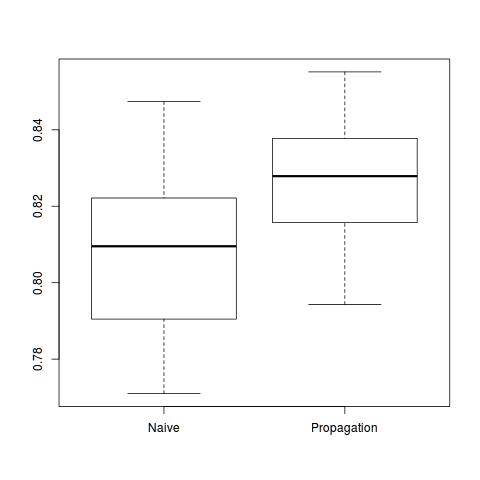
\includegraphics[width=\textwidth]{figures/BRCA_HNCF.jpg}
	\caption{BRCA vs HNCF}
\end{subfigure}
\begin{subfigure}[b]{0.45\textwidth}
	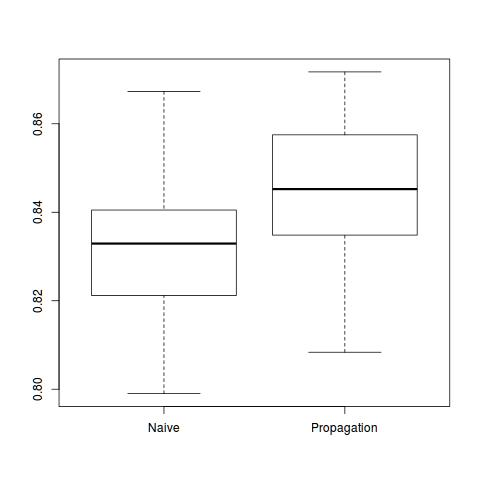
\includegraphics[width=\textwidth]{figures/BRCA_LUAD.jpg}
	\caption{BRCA vs LUAD}
\end{subfigure}
\begin{subfigure}[b]{0.45\textwidth}
	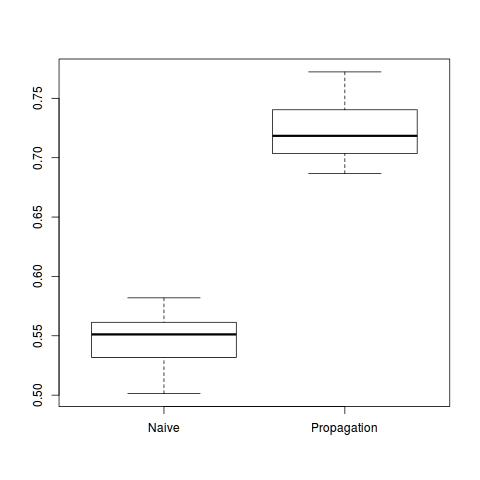
\includegraphics[width=\textwidth]{figures/BRCA_PRAD.jpg}
	\caption{BRCA vs PRAD}
\end{subfigure}
\begin{subfigure}[b]{0.45\textwidth}
	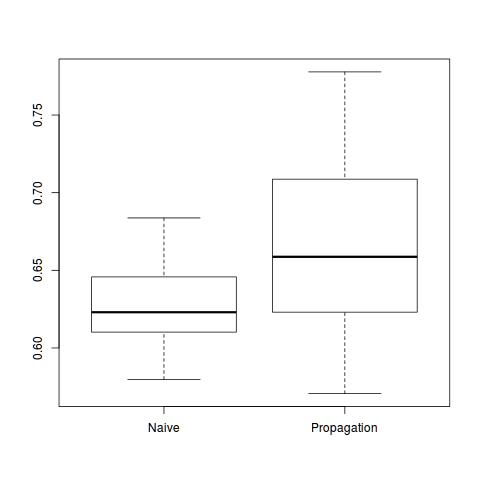
\includegraphics[width=\textwidth]{figures/HNCF_LUAD.jpg}
	\caption{HNCF vs LUAD}
\end{subfigure}
\begin{subfigure}[b]{0.45\textwidth}
	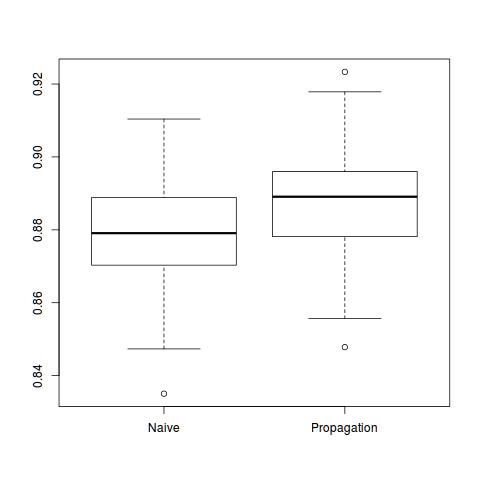
\includegraphics[width=\textwidth]{figures/HNCF_PRAD.jpg}
	\caption{HNCF vs PRAD}
\end{subfigure}
\begin{subfigure}[b]{0.45\textwidth}
	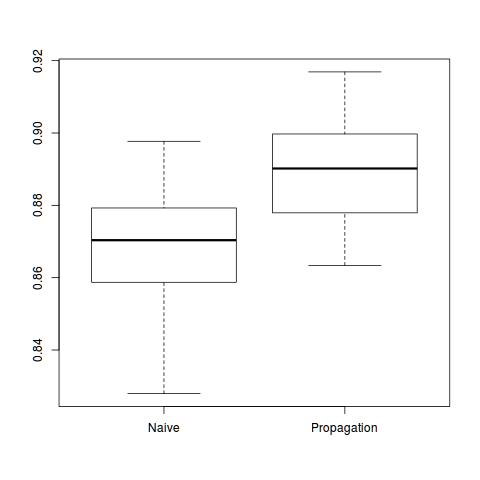
\includegraphics[width=\textwidth]{figures/LUAD_PRAD.jpg}
	\caption{LUAD vs PRAD}
\end{subfigure}
\caption{Comparison between naive classifier and classifier with incorporated
		 protein interaction network. In each experiment we observe an incerase
		 of correct classification rate.
		 For the completeness of the experiment
		 we also performed a classification test with each sample's label 
		 being chosen at random. For each of pairwise comparisons we got 50\% correctness
		 rate, which is expected by chance.}
\label{fig:2-way}
\end{figure}

The results of pairwise comparisons are shown on Figure~\ref{fig:2-way}. As it could
be seen, the network propagation method improves correct classification rate 
for all cases. It is also notable, that the improvement is more significant 
for cases with lower score of initial (naive) calssifier. This suggests that
the described approach is revealing some common pathways that could
not be simply extracted from only genomic data. 

\begin{figure} [h]
\centering
	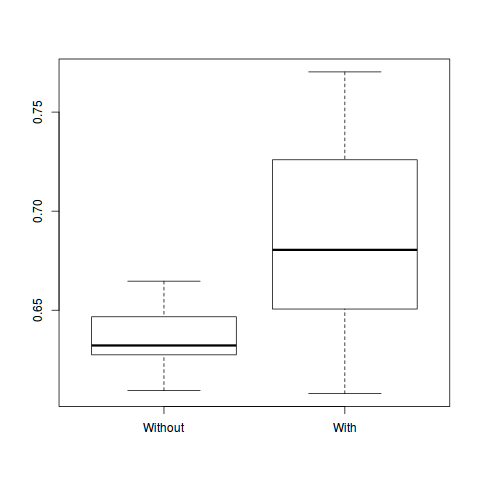
\includegraphics[width=0.5\textwidth]{figures/4-way.png}
\caption{4-way comparison between naive classifier and classifier with incorporated
		 protein interaction network.}
\label{fig:4-way}
\end{figure}

We also performed 4-way comparison between all available samples 
(see Figure~\ref{fig:4-way}). The results also show the better accuracy
of network-based classifier.

\subsection{Revealing discriminative features}

We also performed the analysis of features that are important for classification.
For the \emph{BRCA vs PRAD} comparison we extracted top ten features 
from support vectors of the classifier. The results are shown in Table~\ref{tab:features}.
As it could be seen, some of these important features were not mutated in any of
input samples, which highlights the contribution of network propagation to the
classifier's functionality.

\begin{table}[h]
	\small
    \begin{center}
    \begin{tabular}{c c c c}
	\hline
	ID & Score & Gene & Mutated \\
    \hline
	NBPF10 & -118 & Neuroblastoma breakpoint family, member 10 &  Y \\
	MAP3K1 & 117 & E3 ubiquitin protein ligase & Y \\
	BAGE5 & -101 & B melanoma antigen family, member 5 &  N \\
	BAGE3 & -101 & B melanoma antigen family, member 3 &  N \\
	BAGE4 & -101 & B melanoma antigen family, member 4 &  N \\
	BAGE2 & -101 & B melanoma antigen family, member 2 &  Y \\
	EDRF1 & -95 & Erythroid differentiation regulatory factor 1 &  Y \\
	ARHGAP6 & -93 & Rho GTPase activating protein 6 &  Y \\
	PAX4 & 91 & Paired box 4 &  Y \\
	BPY2B & 87 & Basic charge, Y-linked, 2B &  N \\
    \hline
    \end{tabular}
    \caption{Top ten contributing features of support vectors 
			 in BRCA vs PRAD classification. Score field represents
			 the value of a gene in classification. If a gene is mutated in at least
			 on of the input samples, its state is defined as \emph{mutated},
			 otherwise it is not.}
    \label{tab:features}
    \end{center}
\end{table}
\subsection{Propagation parameters inference}

The performance of network propagation algorithm highly dependends
on the number of iteration and diffusion coefficient $\alpha$. We found that $\alpha = 0.9$
gives the best classification results. Suprisingly, we found that a single iteration 
of network propagation with the given value of $\alpha$ already makes an improvement.
Moreover, for some samples the accuracy rate goes down with the increase of iterations number.
One possible explanation of this might be that the used protein interaction network 
is too general for our purposes and the signal quickly becomes "fuzzy".

\section{Discussion}

In this paper we explre the possibility of protein interaction network to reveal
some discriminative genomic cancer features and describe the experiment to check
this hypothesis. The results show that network propagation method reveal genomic features
that are important for cancer type classification but not directly presented as
somatic mutations.

\end{document}
